

\section{Development of Fastcat Hybrid Monte Carlo Simulator}

\begin{figure}[!ht]
   \begin{center}
   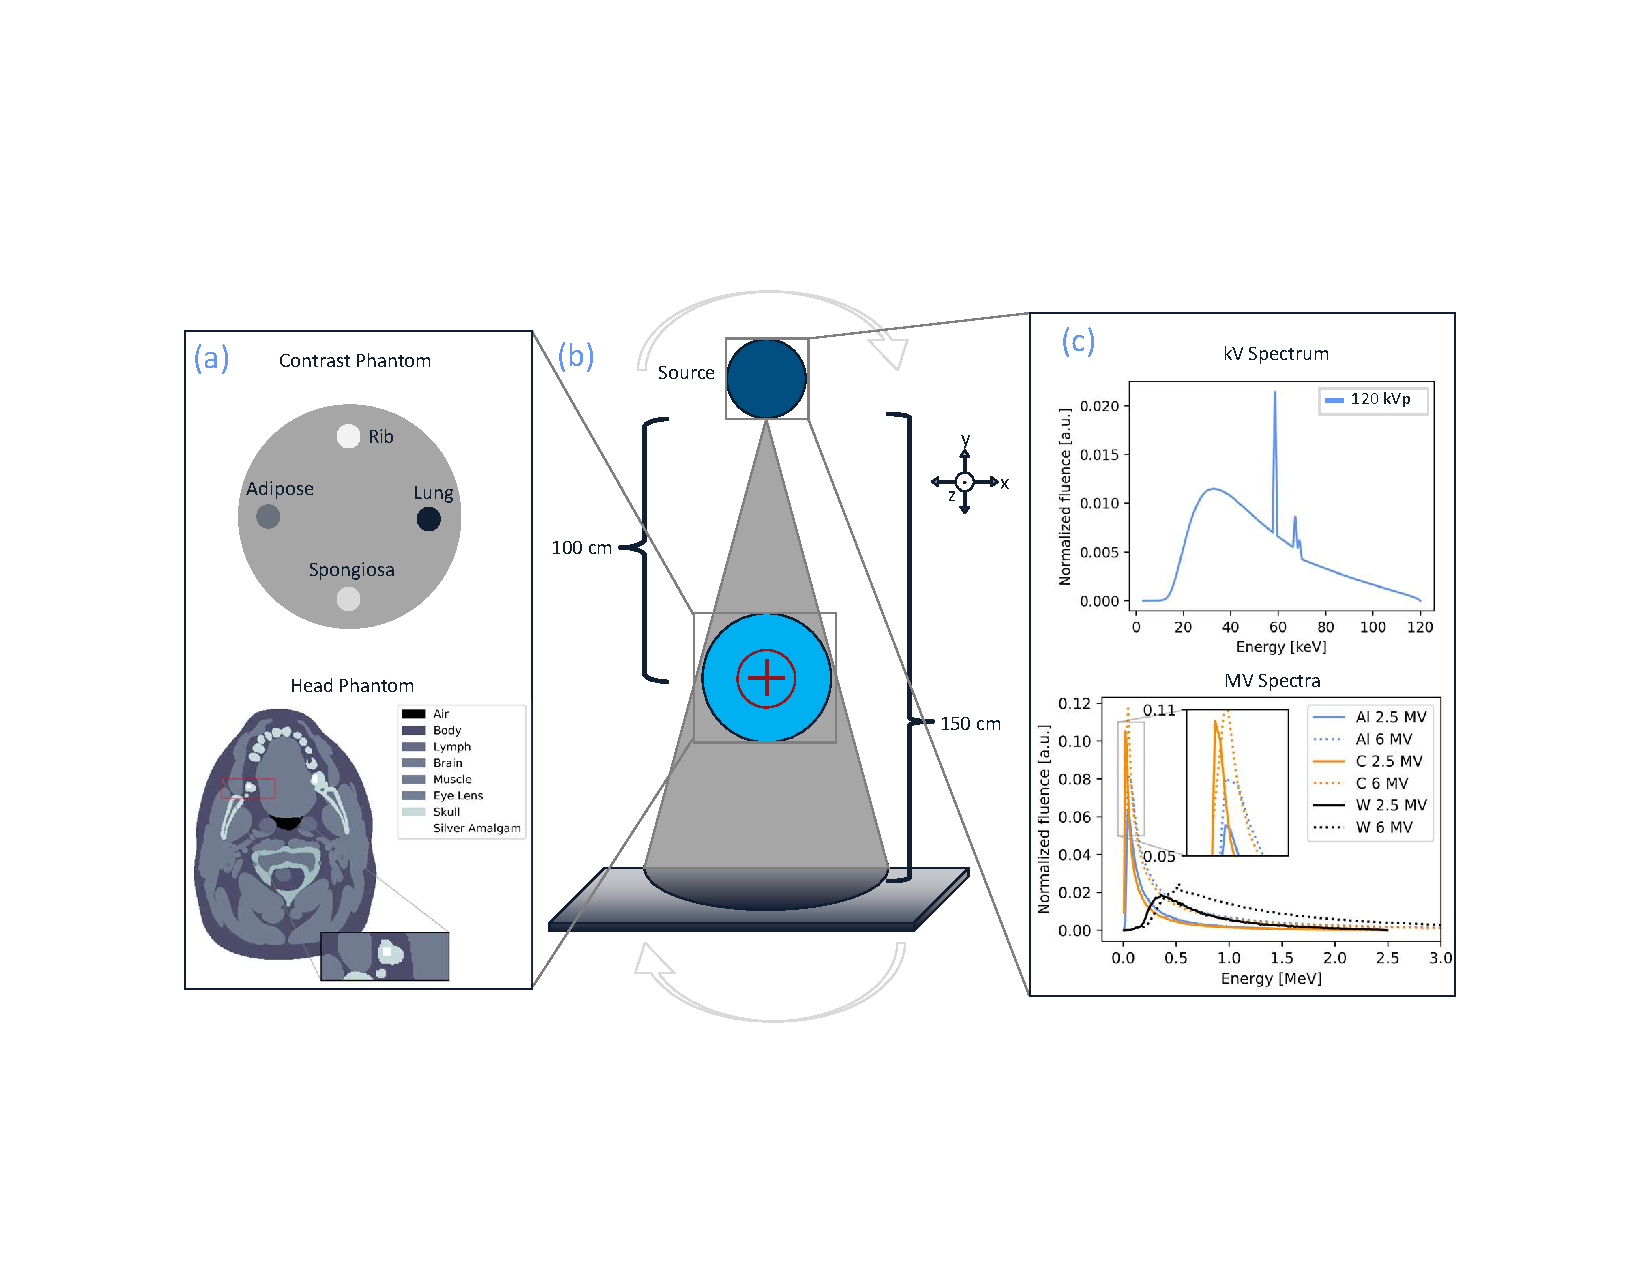
\includegraphics[width=\textwidth,trim={3cm 4cm 2.8cm 4cm}, clip]{figures/Figure_1.pdf}
   \caption{
   An overview of the simulation setup. a) The two phantoms used in this work, the Catphan 515 (top) and the XCAT anthropomorphic head phantom (bottom). b) The simulation geometry. c) The MV energy spectra. d) A slice of the CWO (left), GOS (center), and CsI (right) detectors with component labels corresponding to Table \ref{tab:detector parameters}.
   \label{fig_setup_mtf} 
    }  %note label inside caption
    \end{center}
\end{figure}


\subsection{Fastcat Despription}

The Fastcat simulation tool consists of a number of components that are described below. Fastcat is written in python (version 3.6). A Fastcat simulation can be specified and run as a python script. Likewise, the Fastcat graphical user interface (GUI) can be used to create and run Fastcat simulations. Fastcat incorporates code from xpecgen \cite{Hernandez2016Xpecgen:Anodes}, an open source x-ray tube spectrum generator. The Fastcat default simulation geometry is depicted in Figure \ref{fig_setup_mtf}: A cone beam collimated to 16$\times$16 cm$^2$ at isocenter impinges on a 16 cm diameter cylindrical phantom at a source-to-axis distance (SAD) of 1.00 m and a source-to-detector distance (SSD) of 1.52 m. The GUI workflow is depicted in Figure \ref{fig_overview}, which also shows the user selected parameters.

\subsubsection{Imaging Beam}

Fastcat can use MV or kV x-ray beams for CBCT image generation. MV spectra were calculated with EGSnrc/BEAMnrc \cite{IKawrakow2018TheTransport} using a variety of target materials (carbon, aluminum, and tungsten) and electron beam energies (2.5 and 6 MeV) (Figure \ref{fig_setup_mtf}c). To generate the spectra a mono-energetic 0.02 mm diameter electron beam was incident on the target material. The thicknesses of the target materials were based on existing experimental beams for the carbon and aluminum targets \cite{Flampouri2002OptimizationExperiment} and are summarized in Table \ref{tab:targets_cwo}. For the low atomic number ($Z$) beams (carbon and aluminum), a 2 cm polystyrene filter placed at 50 cm from the target was used to reduce electron fluence in the beam. The photons were collimated by both primary and secondary collimators to create a 10$\times$10 cm$^2$ field size at isocenter and phasespace files were scored at a distance of 100 cm from the target. Global electron and photon cutoffs were set to 0.01 and 0.001 MeV in the BEAMnrc simulations. 1.5$\times$10$^8$ histories were used in each run resulting in 1$\times$10$^6$ to 3$\times$10$^7$ photons in the phasespace file. These simulations took on average 35 core-hours on an Intel Skylake CPU.  Energy spectra with 200 evenly spaced energy bins between 0 and the maximum energy were generated from the phasespace files for input into Fastcat (Figure \ref{fig_setup_mtf}c). The kV spectrum was modelled for a 120 kVp beam with a 12$^\circ$ tungsten anode, a 0.4 mm beryllium window, and 1 mm aluminum filter in xpecgen \cite{Hernandez2016Xpecgen:Anodes}.

\begin{table}[ht]
\begin{center}
\caption{Electron target thicknesses used for the generation of the MV imaging beams.}
\vspace*{1ex}
\label{tab:targets_cwo}
\begin{tabular}{llll}
 \hline
       & tungsten & aluminum & carbon \\  \hline
2.5 MV & 2.3 mm   & 6.7 mm \cite{Parsons2014AVirtuaLinac} & 7.6 mm \cite{Parsons2012BeamTargets}\\
6 MV   & 5 mm     & 8 mm \cite{Baek2019AssessmentFilter}     & 9.9 mm \cite{Parsons2012BeamTargets}
\end{tabular}
\end{center}
\end{table}

\subsubsection{Detector Simulation \label{sec:det}}

Fastcat currently employs two MV detectors: a novel Cadmium Tungstate (CWO) detector\cite{Star-Lack2015AImaging}  and a Gadolinium Oxysulfide (GOS) AS1200 detector\cite{Shi2018APerformance} (both Varian Medical Systems, Palo Alto, CA).  A detector schematic is depicted in Figure \ref{fig_setup_mtf}d and detector material parameters are summarized in Table \ref{tab:detector parameters}.  The CWO detector has pixel septa between crystals and has a pixel pitch of 0.784 mm. The GOS detector has no septa and pixel pitches are set by the active matrix flat-panel imager (AMFPI) pixel pitch. AMFPI pixel pitches of 0.784, 0.392 or 0.336 mm were modelled for the GOS detector and 0.784 and 0.392 mm were modelled for the CWO detector. 
The response of the three detectors, including the optical transport, was simulated in Geant4 \cite{Agostinelli2003Geant4Toolkit} using the Topas \cite{Perl2012Topas:Applications} wrapper.
The responses of the detectors were modelled using a modification of the fastEPID framework developed by Shi \textit{et al.}\cite{Shi2019ADetectors.}. Mono-energetic pencil beams of energies of 10 to 90 keV in 10 keV increments, 100 to 900 keV in 100 keV increments, and 1, 2, 4, and 6 MeV were used to calculate the optical spread function (OSF) as well as the energy deposition efficiency ($\eta$) of each detector. For each of the energies, 1$\times$10$^6$ histories were simulated resulting in a run time of roughly 48 core-hours per detector on an Intel Skylake CPU for the GOS detector. The other detectors had comparable run times but took longer to load the complex CWO pixels and columnar CsI geometries, which took 2 and 6 hours to load, respectively. All Topas simulations used the Geant4 Penelope physics list as well as the Geant4 optical physics list with a particle range cutoff of 5 $\mu m$ for all particles. No variance reduction techniques (VRTs) were used.

 The kV CsI detector in this study was modelled as a 450-$\mu$m CsI scintillating detector\cite{Sharma2012EffectiveGlasses} (Radiation Monitoring Devices, Inc., Water-town MA).  The scintillating crystal is composed of a 100 $\mu$m graphite substrate, 90 $\mu$m of homogeneous CsI, and 360 $\mu$m of columnar CsI (Figure \ref{fig_setup_mtf}d). The columnar CsI was simulated with a column diameter of 10.2 $\mu$m and an 85\% packing density with nitrogen gas between columns. Optical properties are summarized in Table \ref{tab:detector parameters}. All MC simulation settings were the same as stated above for the CWO and GOS detectors. To reduce computation time in all detector simulations, scintillation yields of 600 photons per MeV were used.


\begin{table}[]
\caption{Detector optical parameters
\cite{Star-Lack2015AImaging,Shi2018APerformance,Freed2009ExperimentalScreens}}
\label{tab:detector parameters}
\begin{tabular}{llllll}
\hline
                       & \begin{tabular}[c]{@{}l@{}}Density\\ (g/$cm^3$)\end{tabular} & Material                & \begin{tabular}[c]{@{}l@{}}Thickness\\ (mm)\end{tabular} & \begin{tabular}[c]{@{}l@{}}Abs. l. (cm) $|$\\ Refr. ind.\end{tabular} & \begin{tabular}[c]{@{}l@{}} Refle- \\ ctivity \end{tabular}\\ \hline
(1) carbon Fiber       & 1.62                                                         & C                       & 2.5                                                      & --                                                                              & --           \\
(2) Foam               & 0.05                                                         & C                       & 33.1,25                                                & --                                                                              & --           \\
(3) Vikuiti ESR        & 1.05                                                         & CH                      & 0.065                                                    & 0.01                                                                            & 0.98         \\
(4) Scintillator Pixel & 7.9                                                          & CdWO$_4$                & 15                                                       & 125 $|$ 2.25                                                                    & --           \\
(5) Pixel Glue         & 1.0                                                          & Epoxy                   & 15                                                       & 100 $|$ 1.47                                                                    & --           \\
(6) Pixel Septa        & 2.7                                                          & Al Mylar                & 15                                                       & 0.001                                                                           & 0.88         \\
(7) Meltmount Glue     & 1.0                                                          & CHClO & 0.01                                                     & 300 $|$ 1.7                                                                     & --           \\
(8) Mylar              & 1.38                                                         & C$_{10}$H$_8$O$_4$      & 0.065                                                    & 100 $|$ 1.65                                                                    & --           \\
(9) AMFPI              & 2.6                                                          & SiO$_2$                 & 1                                                        & 0.001 $|$ 1.70                                                                  & --           \\
(10) Fiberglass        & 1.85                                                         & SiO$_2$                 & 0.6, 6.0                                                  & --                                                                              & --           \\
(11) Copper buildup    & 8.9                                                          & Cu                      & 1                                                        & --                                                                              & --           \\
(12) GOS phospor       & 4.59                                                         & GdOS:Tb         & 0.29                                                     & 43 $|$ 2.3, 1.0                                                       & --           \\
(13) Al alloy          & 2.8                                                          & Al                      & 1                                                        & --                                                                              & --           \\
(14) Pb alloy          & 10.95                                                        & Pb                      & 3                                                        & --                                                                              & --           \\
(15) Graphite          & 2.26                                                         & C                       & 1                                                        & 0.001                                                                           & 0.88         \\
(16) CsI               & 4.51                                                         & CsI:Tl                  & 0.9                                                      & 1.25 $|$ 1.8                                                                    & --           \\
(17) Columnar CsI      & 4.51                                                         & CsI:Tl                  & 3.60                                                     & 1.25 $|$ 1.8                                                                    & --          
\end{tabular}
\centering
\vspace*{2ex}
\end{table}


As stated above, Topas MC simulations were used to determine the OSF and $\eta$ of each detector. The OSF is defined as

\begin{equation}
    OSF(i,j) = \frac{Output(i,j)}{N_{incident}\times\eta},
\end{equation}

\noindent where $Output(i,j)$ is the number of optical photons incident on the readout pixel with row and column indices of $i$ and $j$ and $N_{incident}$ is the total number of photons incident on the detector.

In this work, the OSFs were used to generate a detector modulation transfer function (MTF) from the point spread function (PSF). The 2D energy dependent OSFs were weighted by energy deposition efficiency multiplied with the incident spectrum from the selected beam to estimate the hypothetical PSF. This weighting is a modification of fastEPID. In fastEPID each photon is individually accepted or rejected from the detector with probability $\eta$. In Fastcat the fluence at a given energy is weighted directly by $\eta$. This approximation is done as the photons are not transported individually in Fastcat. This PSF was then convolved with an idealized 0.3 mm wide slit tilted at 2.5$^\circ$ to generate a line spread function (LSF), that was then presampled to estimate the MTF. The OSF was also used in the Fastcat CBCT simulation to generate the detector response, as discussed in section II.C. 
 
 \subsubsection{Scatter Modelling \label{sec:scat}}

The scatter kernels for a 16-cm diameter water phantom were generated in Topas using 18 mono-energetic cone beams and the default simulation geometry. To generate the scatter kernels a phasespace file was collected at the surface of a 40$\times$10$\times$0.3 cm$^3$ air slab located at the 1.52 cm SDD. Photons that did not interact in the phantom were filtered out. The spatial distribution of the scattered particles $y$ was averaged in the $z$ direction and fitted to a two parameter curve-fit of the form:

\begin{equation}
    y = (\frac{a}{\sqrt{x^2 + a^2}})^b,
\end{equation}

where $a$ and $b$ are fitting parameters and $x$ is the off axis distance. This fit was used to ensure a symmetric fit, and it resulted in a root mean squared error lower than a symmetric polynomial fit. The resultant energy distribution of the scatter from each mono-energetic cone beam was neglected in the analysis as sufficiently close agreement was seen when approximating the scatter as mono-energetic. These mono-energetic cone beam scatter curves were then combined with analytical projections to form the CBCT projection data discussed below.

\subsubsection{Raytracing}

The bulk of the computational work of Fastcat CBCT image generation is in the CBCT raytracing. In this work the TIGRE \cite{Biguri2016TIGRE:Reconstruction} GPU reconstruction package was used for generating the cone beam forward projections. These primary projections, are denoted as “projections” and they are equivalent to the sum of attenuation coefficient along the path of the ray between the source and detector. This is to be distinguished from what we will call the “intensity profiles” which are the counts in a given detector pixel. 

One forward projection is calculated for each CBCT projection for each of the 18 energies. These primary projections are converted to intensity profiles using a flood field intensity profile made with the same geometry and number of photons as the scatter kernels, ensuring the correct scaling of the scatter. The scatter kernels are then added to the primary intensity profiles. These complete intensity profiles, $I(E)$, are then weighted by the fluence $\phi(E)$ and energy deposition efficiency $\eta(E)$ to form the final intensity $I_f$ as

\begin{equation}
    I_f = \sum\limits_{E} \phi(E) \eta(E) I(E)
\end{equation}

 To reduce computation time only ten slices in the z direction are simulated in the default phantoms, 512$\times$512$\times$10 voxels with voxel sizes of 0.31$\times$0.31$\times$0.31 mm$^3$ were used for the Catphan 515. Likewise, the XCAT phantom had dimensions of and 1024$\times$1024$\times$10 voxels with voxel sizes of 0.5$\times$0.5$\times$3.125 mm$^3$.

\subsubsection{Noise and CBCT reconstruction}

Noise is added through a Poisson scaling of the particle counts incident on the detector. This scaling can be related to either dose or particle fluence as will be discussed below. The intensity profiles are then convolved with the OSF at each energy and summed to create the final profile at each beam angle. These are converted back to projections using the corresponding flood field and reconstructed. Reconstructions are performed with TIGRE algorithms which have many options for reconstruction types including the default FDK reconstruction \cite{Feldkamp1984PracticalAlgorithm} and more advanced iterative reconstruction. CBCT images were converted into Hounsfield Units (HU) using water region of the phantom for normalization. Image analyses can then be done using specific analysis modules attached to each phantom. For the Catphan 515 module, contrasts and contrast to noise ratios can be calculated. CNR was calculated as 

\begin{equation}
    CNR = \frac{|HU_w - HU_{ROI}|}{\sqrt{\sigma_w^2 + \sigma_{ROI}^2}}
\end{equation}

\noindent Where $HU_w$ and $HU_{ROI}$ are the HU values water and the region of interest (ROI) and the regions respective standard deviations are represented by the $\sigma$s.

\subsubsection{Dose calculation}

The scaling of the noise in the simulation can be determined by the user based on either the requested mean dose to the phantom or the total particle fluence. Noise defined by particle fluence scales the intensity profile as $H$:

\begin{equation}
\label{nphot}
    H = \frac{N_\gamma}{A/A_p},
\end{equation}

where $N_\gamma$ is the total number of particles $A$ is the area of the beam and $A_p$ is the area of a detector pixel. Once $H$ is foun.  Assumption of uniform phantom scatterd the flood field is scaled to that height before converting the projections to intensity profiles. Noise is then added using Poisson scaling based on the number of counts in a pixel.  

Another option is to provide the mean dose to the water phantom for one projection. Fastcat will then estimate the noise based on the dose provided. Fastcat's dose estimate is based on the collision kerma in the phantom. This value for collision kerma is then related to dose by an empirical correction factor. This factor accounts for charged particle disequilibrium in the phantom. The dose calculation is as follows: The initial collision kerma per particle ($K_0$) at each energy is calculated as

\begin{equation}
    K_0(E) = \frac{1}{N_i M}\sum\limits_i E \frac{\mu_{en}(E)}{\mu(E)} (1 - e^{-\mu_i(E) x_i}),
\end{equation}

\noindent where $i$ is the ray index, $\mu$ and $\mu_{en}$ are the linear and energy-absorption coefficients of water, respectively, $N_i$ is the number of rays, and $M$ is the mass of the phantom. These values estimate the average dose per particle at each energy. These initial collision kermas are weighted by the selected fluence $\phi$ and summed to get a total collision kerma $K_p$ per particle

\begin{equation}
  K_p = \sum\limits_{E} \phi(E) K_0(E).
\end{equation}

\noindent These collision kerma estimates per particle were seen to correlate linearly (R$^2$ $>$ 0.99) with the mean dose per particle calculated in Topas for the 16 cm diameter water phantom. An empirical linear fit to the Topas doses was used to relate the collision kerma to the final dose estimate per particle. 

The noise was then calculated based on the number of particles. This was achieved by dividing the requested dose by the dose per particle. With the number of particles known, equation (\ref{nphot}) was used to calculate the noise. The dose calculations were validated by comparing the average dose to the Catphan 515 phantom estimated in Fastcat to the dose calculated using the same imaging setup in Topas.

\subsubsection{Bowtie and Flattening Filters}

Additional models in Fastcat are applied to model some features of experimental scans. The kV bowtie filter was known to have a minimum thickness of 1.53 mm aluminum and a maximum thickness of 27.3 mm aluminum. The proprietary bowtie filter shape was unknown and estimated from the shape of a kV OBI air scan. With Fastcat’s model of the kV imager spectra and the energy response of the detector, a weighted attenuation coefficient of aluminum was calculated for the kV OBI. This attenuation coefficient was then used to estimate the thickness of aluminum filtration present at each pixel. While an additional thickness of 1.53 mm of aluminum was added to each pixel to account for the base thickness of the bowtie filter. The maximum thickness of aluminum was calculated to be 28.3 mm using this method. This thickness is seen to be nearly equivalent to the specified thickness plus an additional factor accounting for a non-perpendicular path through the filter. Fastcat’s kV beam was then filtered by the calculated amount of aluminum at each pixel during simulation. Additionally, the MC scatter for the kV image was recalculated to include the bowtie filter’s effect on scatter. To account for the heel effect in the beam, tungsten filtration in the shape of a linear ramp increasing in the cathode-anode direction with a maximum height of 0.1 mm was added.

The thickness of the MV flattening filter was also estimated. In this case, the Fastcat beam was attenuated by a gaussian tungsten flattening filter. The height and standard deviation were chosen such that a profile through the reconstructed CBCT best matched experimental CBCTs.

\subsubsection{Anti-scatter Grid}

To correctly model the kV OBI a model for the anti-scatter grid (ASG) was introduced. The model is based on measurements made by Wiegert \textit{et al.} \cite{Wiegert2004PerformanceCT} Primary transmission factor and scatter transmission factors from the 44r10 ASG discussed in the paper were used. These factors are 0.76 and 0.37, respectively. Primary fluence reaching the detector in the Fastcat simulation was multiplied by the primary transmission factor. The scatter transmission factor was used to separate the scatter into two portions handled by the simulation as either accepted or attenuated, respectively. The first portion was accepted by the detector while the second portion was assumed to be incident on the ASG at a 12 degree angle. Where 12 degrees was the mean angle of scatter incidence from Weigert \textit{et al.}’s work. This second portion was filtered by 173 $\mu$m of lead, which is the path length through the 36 $\mu$m lamella at an angle of 12$^\circ$. The number of particles in these two portions were calculated such that the total Fastcat scatter transmission factor agreed with the theoretical.

\subsubsection{Virtual Catphan Phantom}

 A virtual version of the Catphan phantom was created. The virtual phantom was voxelized into 1024 pixels horizontally (h) 1024 pixels vertically (v) with voxel dimensions of 0.195 mm (h), (v) and a slice thickness of 0.313 mm. The slice thickness was made larger than axial voxel dimensions as the phantom is cylindrically symmetric and the slice thickness has no effect on simulation results. Materials linear attenuation coefficients were calculated using the material compositions and densities in the Catphan documentation. Densities of Delrin and the inner and outer body materials of the phantom were estimated as data was not available on their exact composition. Delrin’s composition was estimated to match the attenuation coefficient available on the manufacturer site. The two body materials were estimated using the composition of acrylic and densities that would give the materials the relative electron densities reported in Star-Lack \textit{et al.} \cite{Star-Lack2015AImaging}.
 
\subsection{Fastcat Validation}
 
\subsubsection{Experimental Data Acquisition}

\begin{figure}[h!]
  \begin{center}
  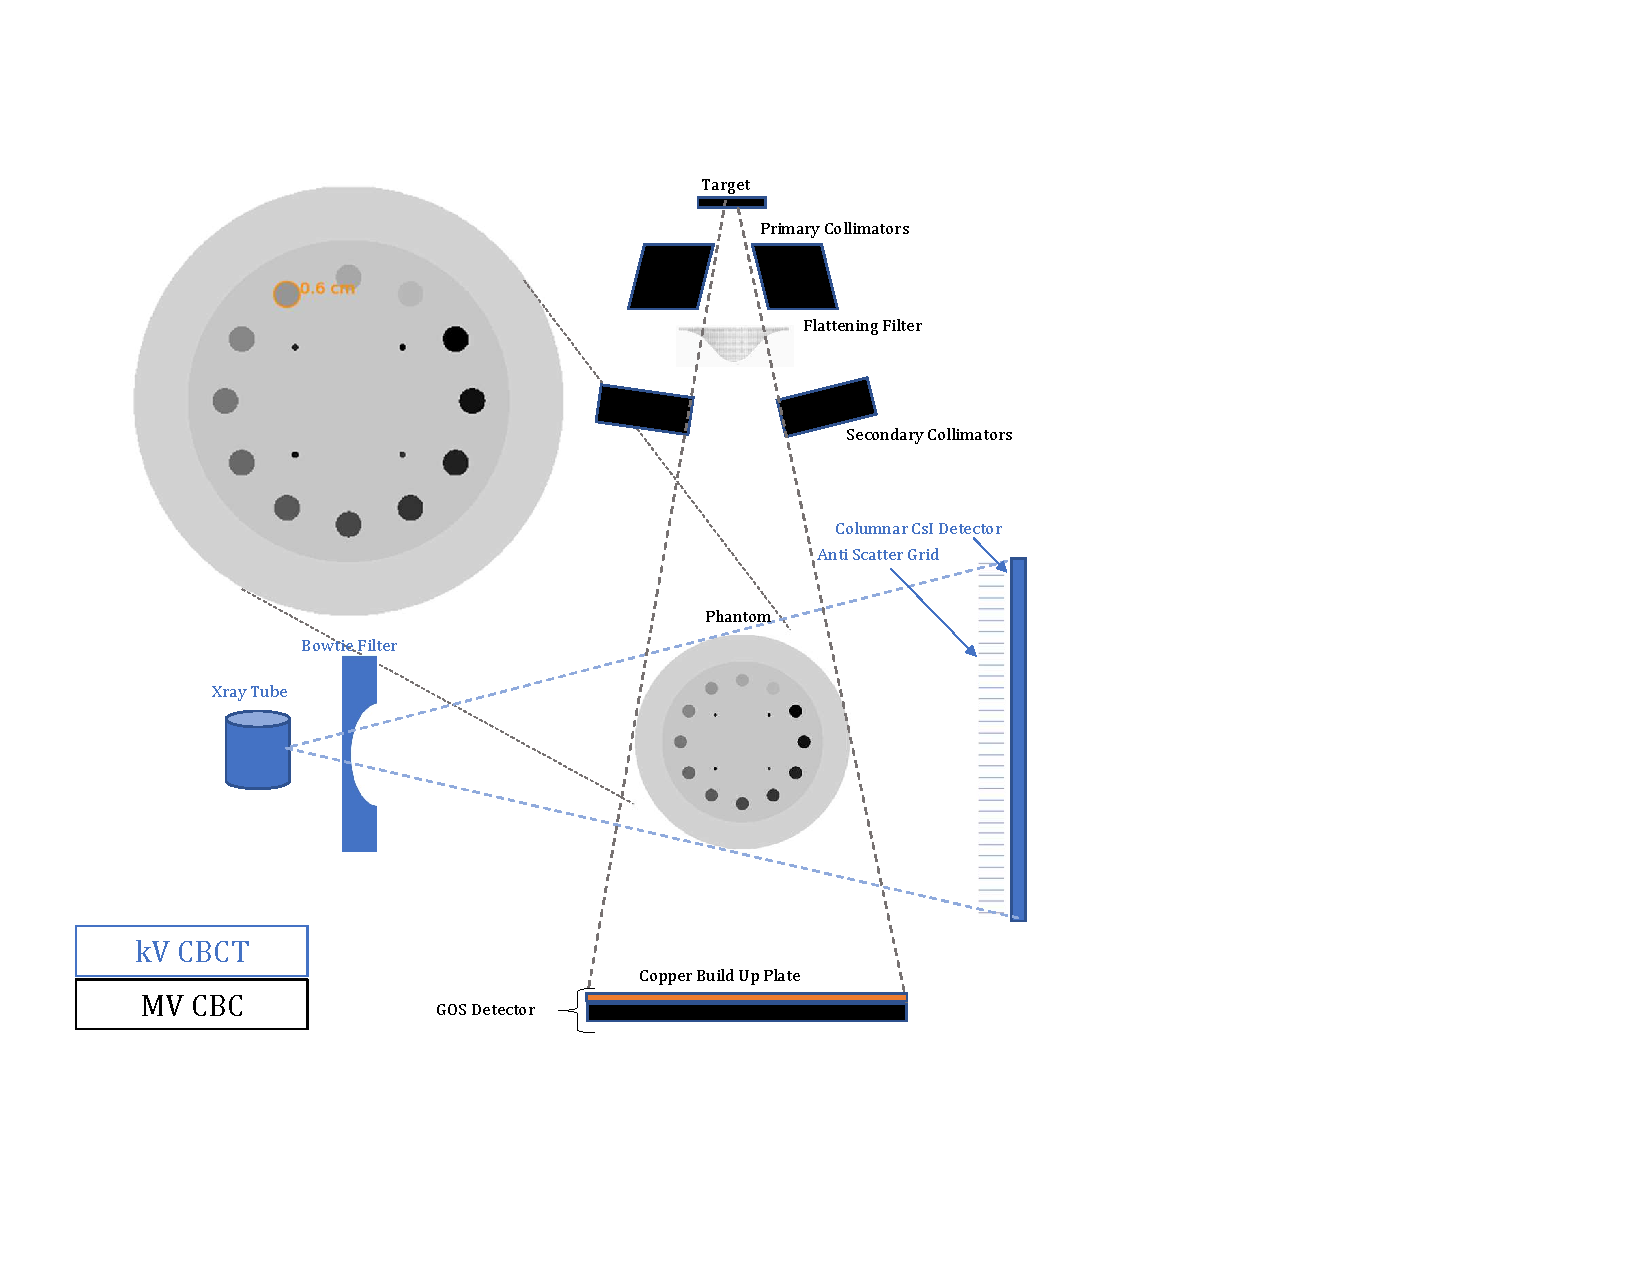
\includegraphics[width=0.75\textwidth,trim={1cm 4cm 9.5cm 2cm}, clip]{figures/setup_figure.pdf}
  \caption{
  A schematic of the Truebeam linac and CTP404 module. The kV and MV imaging systems are shown in blue and black, respectively. Dotted lines outline where the beams would be generated. The phantom displayed is used to represent the phantom geometry. Thus, the phantom colormap does not correspond to any material property. The schematic is not to scale. 
  \label{fig_setup_val} 
    }  %note label inside caption
    \end{center}
\end{figure}


Fastcat was validated for two different experimental CBCT data sets acquired on a Truebeam STx linac (Varian Medical Systems, Palo Alto, CA).

\subsubsection{kV CBCT}

An experimental kV CBCT image was acquired using the Varian Truebeam kV Planar Imager (which we also refer to as the OBI). The kV CBCT image was acquired using a Varian GS-1542 x-ray tube with a 100 kVp x-ray beam. The spectra was filtered by 2.7 mm aluminum inherent filtration as well as a 0.89 mm titanium beam hardening filter. An aluminum bowtie filter was also used with a minimum thickness of 1.53 mm and a maximum thickness of 27.42 mm. The detector was a PaxScan 4030CB (Varex Imaging Corporation) flat panel detector with an anti-scatter grid (ASG). The ASG was the default model with a grid ratio of 10, septal thickness of 0.036 mm, and line density of 60 lines/cm. The detector itself was a 0.6 mm columnar CsI detector with a fill factor of 70\% and an amorphous silicon readout pitch of 194 $\mu$m. The scan was acquired in the fluoro-mode with pixels binned to 388 $\mu$m. Thus, the detector had a pixel matrix of 1024$\times$768, with a total detector size of 397$\times$298 mm. A total of 887 views of the phantom were acquired at equally spaced angles over a 360 degree rotation. The beam was collimated to 14 cm $\times$ 14 cm at isocenter. The scan CTDI$_{vol}$ was 21.1 mGy. The CBCT was acquired in developer mode and the reconstruction was performed using the FDK algorithm \cite{Feldkamp1984PracticalAlgorithm} with a ram-lak filter. The reconstruction kV CBCT image size was 512$\times$512 pixels with isotropic voxel dimensions of 0.391 mm$^3$.

\subsubsection{MV CBCT}

The MV CBCT was acquired using the 6 MV therapy beam with the default tungsten target and a flattening filter. The detector used was a Varian as1200 GOS detector with a pixel pitch of 0.392 mm. Optical properties of the detector are described in more detail in the work of Shi \textit{et al.} \cite{Shi2018APerformance}. The detector had a pixel matrix of 1024$\times$768, with a total detector size of 401$\times$301 mm. A total of 493 views of the phantom were taken at equally spaced angles over a 360 degree rotation. The beam was collimated to 14 cm $\times$ 14 cm at isocenter. The scan was acquired with a dose of 300 MU. A high dose was used to ensure adequate image quality from the low quantum efficiency GOS detector. It should be noted that 300 MU is much too high for a clinical MV CBCT dose and was only used for validation. The CBCT was acquired in developer mode and the reconstruction was performed using the FDK algorithm with a ram-lak filter. The reconstructed CBCT image size was 512 $\times$ 512 pixels with isotropic voxel dimensions of 0.391 mm$^3$. An fft-wavelet ring artifact reduction was used to reduce artifacts in the presented image \cite{Munch2009StripeFiltering}. Ring artifact reduction was not used in the analysis since the dampening of high wavelet frequencies can reduce image noise.

\subsubsection{Validation Metrics}

\subsubsection{Detector MTF}

Detector modulation transfer function (MTF) was measured using a slanted virtual slit of 0.3 mm in Fastcat. The method of measuring the detector MTF is discussed in previous work \cite{OConnell2021FastCAT:Simulation}. Detector MTF was compared to experimental results from previous works of Howansky \textit{et al.} and Shi \textit{et al.} \cite{Howansky2017DirectImaging,Shi2018APerformance}.

\subsubsection{CBCT Contrast, CNR, and NPS}

To validate Fastcat, image quality was compared between Fastcat and experimental images. Original units of attenuation coefficients in cm$^{-1}$ for both images were first converted to Hounsfield Units (HU) by subtracting the CT value of water in the image and scaling by the difference between water and air regions in the image. 

\begin{equation}
HU = 1000 \frac{im - \mu_{water}}{(\mu_{water} - \mu_{air})}
\end{equation}
                   
Where $im$ is the reconstructed image and $\mu_{water}$ and $\mu_{air}$ are the linear attenuation coefficients of water and air, respectively. For Fastcat, water values were taken from a separate scan of a water phantom. Contrast was compared using regions of interest (ROIs) in each insert of the CTP404 sensiometry module. Regions of interest were made slightly smaller than the inserts to avoid partial volume effects. The mean value over sixteen slices was used as the contrast value while the standard deviation of the contrast in the sixteen slices was used as an estimate of the standard deviation. Contrast to noise ratio (CNR) was measured using the same ROIs. The standard deviation of each ROI was used as an estimate of the noise. Contrast, again, was measured against water, the CNR was then

\begin{equation}
CNR = \frac{\mu_{ROI} - \mu_{water}}{\sigma_{ROI}}
\end{equation}

Where $\mu_{ROI}$ and $\sigma_{ROI}$ are the mean and standard deviation of each ROI. CNR was measured in each slice over sixteen slices, with the mean value used as a final estimate of the CNR. The standard deviation of the sixteen slices was used as an estimate of the standard deviation of the CNR.

Radially averaged noise power spectrum (NPS) was calculated using 50 randomly sampled 64 $\times$ 64 pixel regions inside a region of 100 $\times$ 100 pixels at the center of the CTP 404 module for each of the experimental and Fastcat images. NPS was calculated in each slice by averaging the squared 2D Fourier transform radially and the results were averaged over four slices to reduce noise.

\subsection{Simulation Validation of Fastcat}

\subsubsection{Detector MTF}

Fastcat showed very good agreement with measured and simulated MTFs for both the GOS and CWO detectors (Figure \ref{MTF_comparison}). For the GOS detector the average root mean squared error (RMSE) between the Fastcat and Topas simulations was 0.5\%. The maximum RMSE was 1.3\% at an MTF of 0.61 mm$^{-1}$. The average RMSE and maximum RMSE between the GOS MTF calculated by Fastcat and measurement data provided by Shi \textit{et. al} was 1.2\% and 2.8\% at an MTF of 0.67 mm$^{-1}$, respectively. For the CWO detector, the average RMSE between the Fastcat and simulated data of Star-Lack \textit{et al.} was 3.3 \% and the largest discrepancy of  7.9 \% occured at a spatial frequency of 0.64 mm$^{-1}$. The average RMSE between the Fastcat and the measured data of Star-lack \textit{et al.} was 3.5 \% and the maximum RMSE of 7.9 \% was observed at a spatial frequency of 0.64 mm$^{-1}$.

\begin{figure}[t!]
   \begin{center}
   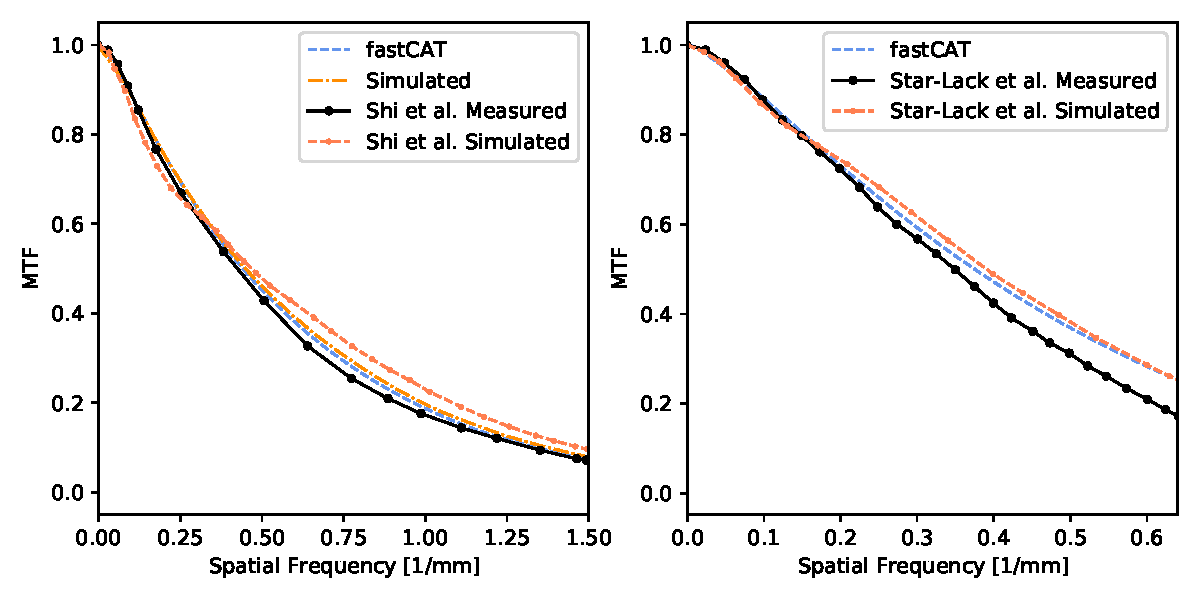
\includegraphics[width=0.9\textwidth]{figures/MTF.pdf}
   \caption{
   (L) A comparison of Fastcat-calculated MTF with measured and simulated values for the GOS detector with a 0.336 mm pixel pitch (based on Shi \textit{et al.})  and (R) for the CWO detector with a 0.784 mm pixel pitch (based on Star-lack \textit{et al.}).
   \label{MTF_comparison} 
    }  %note label inside caption
    \end{center}
\end{figure}


\begin{figure}[ht!]
   \begin{center}
   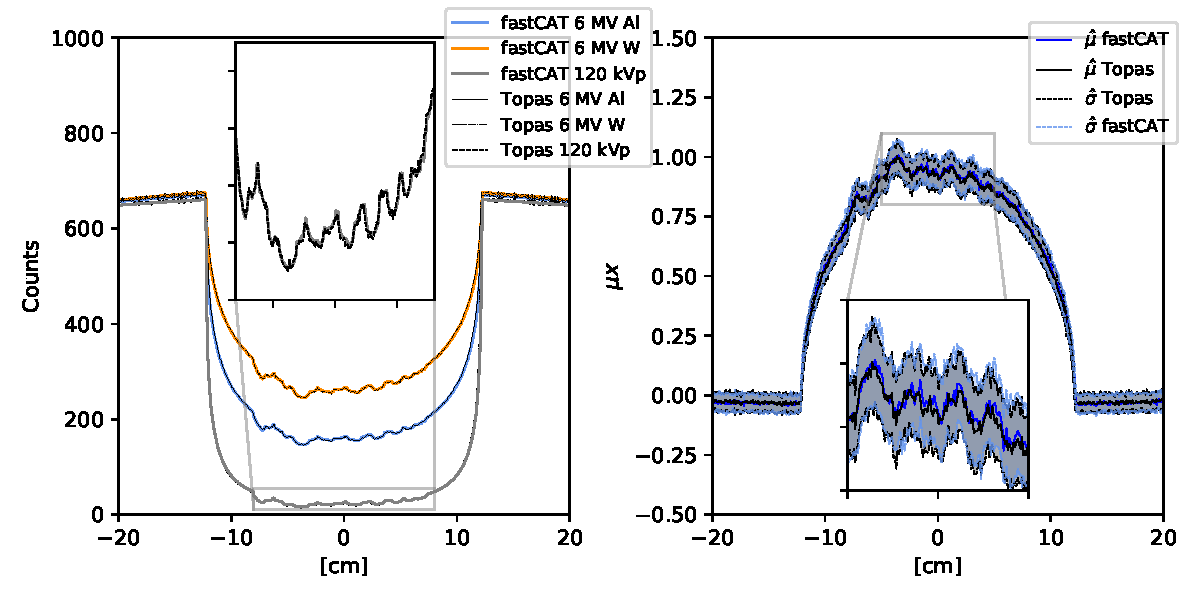
\includegraphics[width=0.9\textwidth,trim={0 0 0 0},clip]{figures/one_slice_comparison_2panel.pdf}
   \caption{
   (L) Comparison of Fastcat and Topas intensity profiles for a 6 MV aluminum beam, a 6 MV tungsten beam, and a 120 kVp x-ray tube beam. (R) Comparison of Fastcat and Topas scatter profiles for a 6 MV tungsten projection (averaged over 64 pixels in the $z$ direction).
   \label{one_slice_comparison} 
    }  %note label inside caption
    \end{center}
\end{figure}

\subsubsection{Projections and dose}

Comparisons of the Catphan 515 phantom projections and intensity profiles as calculated by Fastcat and Topas are shown in Figure \ref{one_slice_comparison}. The intensity profiles for the 6 MV aluminum beam presented in Figure \ref{one_slice_comparison} on the left demonstrated a close agreement between Fastcat and Topas. The Fastcat and Topas intensity profiles had an average RMSE of 0.4\% with a worst case RMSE of 1.1\%.  Likewise, for the 6 MV tungsten beam, Fastcat had an average RMSE of 0.2\% of the Topas values with a worst case RMSE of 1.4\%. The 120 kVp beam Fastcat  intensity profile had an average RMSE of 0.5\% of the Topas values with a worst case RMSE of 1.7\%. The lowest accuracy was likely due to noise in Topas simulations. Fastcat noise showed good agreement with MC noise as seen in Figure \ref{one_slice_comparison} on the right. The RMSE of the standard deviation of all pixels between Fastcat and Topas was 0.21 \% for the 6 MV tungsten beam.

Fastcat imaging dose calculations for the Catphan 515 phantom were compared to dose calculated for the same simulation in Topas. The mean dose to entire phantom was in a good agreement with the Topas dose estimates. Fastcat dose per photon had a mean difference of 1.4\% of the Topas values for all beams. The largest dose estimation error between Fastcat and Topas was for the 2.5 MV carbon beam with an error of 4.5 \%.

\begin{figure}[ht!]
   \begin{center}
   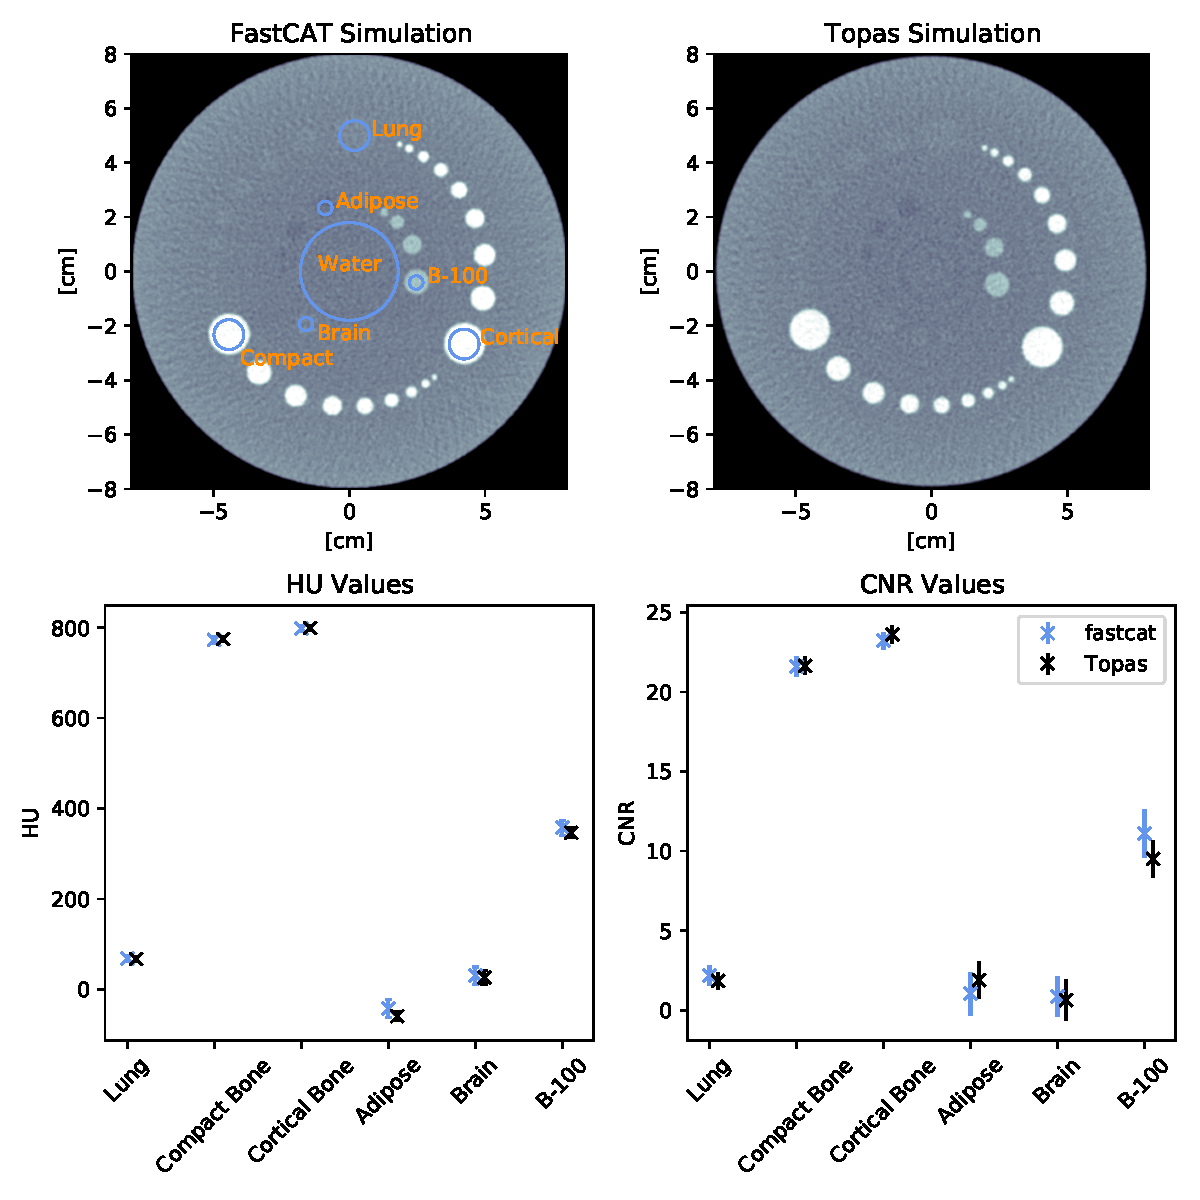
\includegraphics[width=0.9\textwidth]{figures/contrast_4_panel.pdf}
   \caption{
   (Top) Fastcat simulation with ROI placement used for HU and CNR calculations (L) and full Topas simulation of the Catphan 515 phantom (R). (Bottom) A comparison of HU values (L) and CNR (R) in the CBCT Fastcat and Topas reconstruction.
   \label{recon_comparison} 
    }  %note label inside caption
    \end{center}
\end{figure}

\subsubsection{CBCT images, CNR and calculation time}

The agreement in intensity profiles translated into good agreement between HU values in a full CBCT reconstruction of the Catphan 515 phantom (Figure \ref{recon_comparison}). The average RMSE between Fastcat and MC-calculated contrast was 0.5\%. The mean error for each of the inserts was 0.6, -1.4, -1.3, 15.8, 4.2, and 10.2 HU for the deflated lung, compact and cortical bone, adipose, brain and B-100, respectively. All errors were within the 95\% confidence interval.


The good contrast agreement also extended to good CNR agreement between Fastcat and Topas simulations (Figure \ref{recon_comparison}). The average RMSE between Fastcat and MC in terms of CNR was 0.55. The RMSE for the each of the inserts was 0.30, 0.08, 0.39, 0.79, 0.15 and 1.59 for the deflated lung, compact and cortical bone, adipose, brain and B-100, respectively. All errors were within the 95\% confidence interval.

\begin{figure*}[h!]
   \begin{center}
   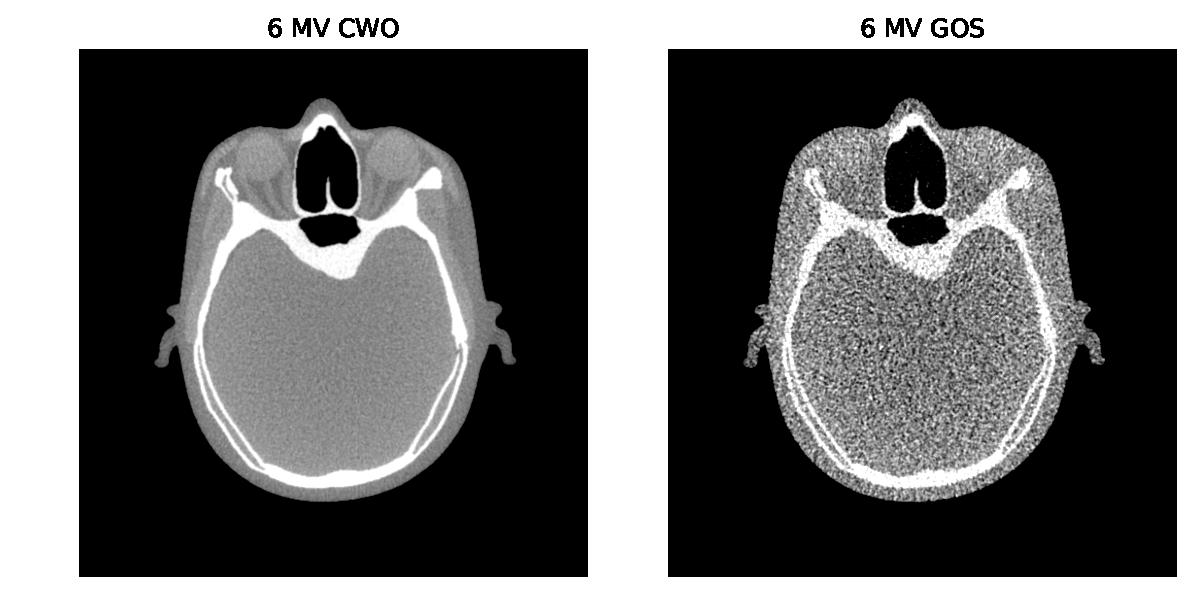
\includegraphics[width=0.8\textwidth,trim={0 0 0 0},clip]{figures/XCATs.pdf}
  \caption{
   Fastcat CBCT images of an anthropomorphic head phantom created with (L) a 6 MV tungsten beam and the CWO detector and (R) a 6 MV tungsten beam and the GOS detector. CBCTs were normalized to a mean dose to the phantom of 7 mGy and used 487 projections.
   \label{XCATs} 
    }  %note label inside caption
    \end{center}
\end{figure*}


To demonstrate Fastcat capability to simulate anthropomorphic phantoms, CBCT images of the head of the XCAT phantom are shown in (Figure \ref{XCATs}). CBCT images presented in Figure \ref{XCATs} can be qualitatively compared to the 6 MV Catphan CBCT images presented by Star-Lack \textit{et al.}\cite{Star-Lack2015AImaging} The increased noise in the GOS image due to the lower DQE of the detector is evident in both cases.

A computational time comparison for CBCT simulations performed with a full Topas MC simulation, fastEPID and Fastcat for a 180-projection CBCT dataset generated with 6 MV tungsten beam was performed. An extrapolation is made for a full Topas MC simulation based on the time for single projection simulation with 10$^9$ photons. The extrapolation predicts 5.6 core-years of compute time to create a full CBCT. A fastEPID simulation using the same parameters would take an estimated 0.32 core-years, while the Fastcat simulations takes 40 and 61 seconds for a 512$\times$512$\times$10 and 1024$\times$1024$\times$10 reconstructed image size respectively.

\subsection{Experimantal Validation of Fastcat}
\subsubsection{CBCT Image Comparison}

\begin{figure}[ht!]
  \begin{center}
  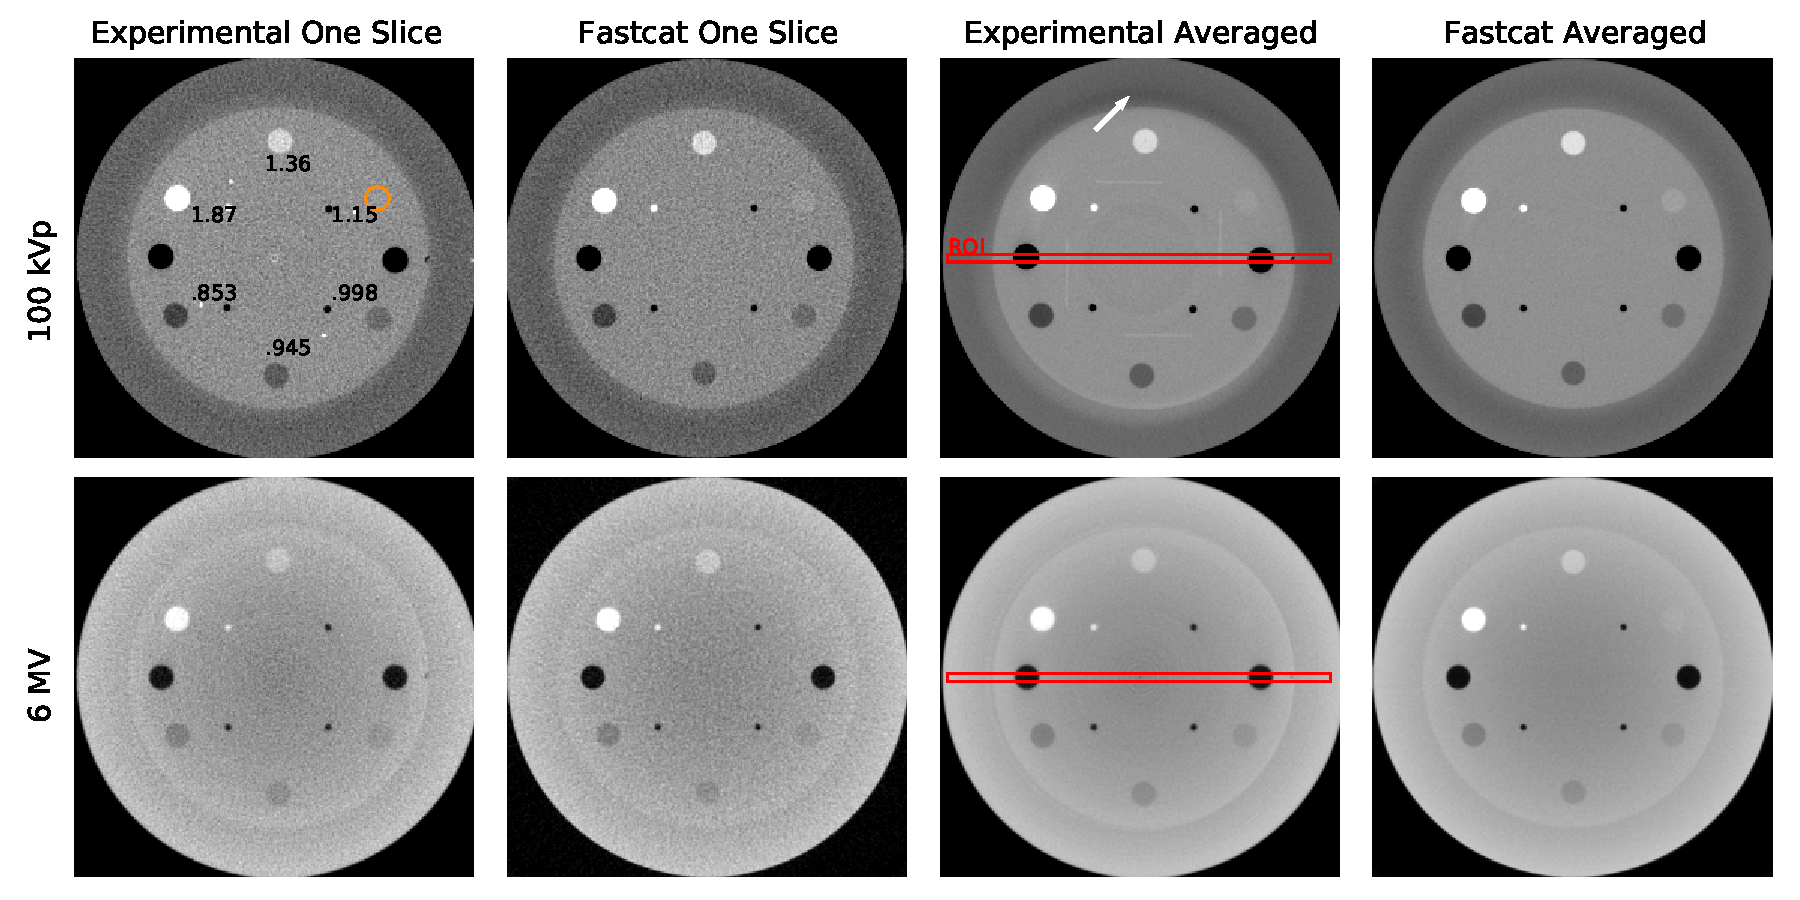
\includegraphics[width=\textwidth, clip]{figures/all_cbcts.pdf}
  \caption{
  A qualitative comparison between experimental CBCTs and Fastcat simulations averaged over 16 slices and for one CBCT slice, respectively. The relative electron densities of the inserts are shown in black. The mean of the ROI shown in red are plotted in Figure \ref{profile}. An arrow indicates a crescent artifact from mechanical misalignment. The small dark spot on the right of the experimental phantom is an alignment marker not included in the Fastcat simulation. Window (W) and level (L) of 1000/300. 
  \label{images} 
    }  %note label inside caption
    \end{center}
\end{figure}

Experimental and Fastcat simulated CBCTs were compared. Figure \ref{images} shows a comparison of 100 kVp and 6 MV experimental and Fastcat images, respectively. Qualitatively, the experimental and Fastcat-simulated CBCT are similar. The effect of the bowtie filter can be seen in the 100 kVp CBCTs which are qualitatively uniform. The effect of the flattening filter can be seen in the 6 MV images where beam hardening artifacts can be seen.

\begin{figure}[ht!]
  \begin{center}
  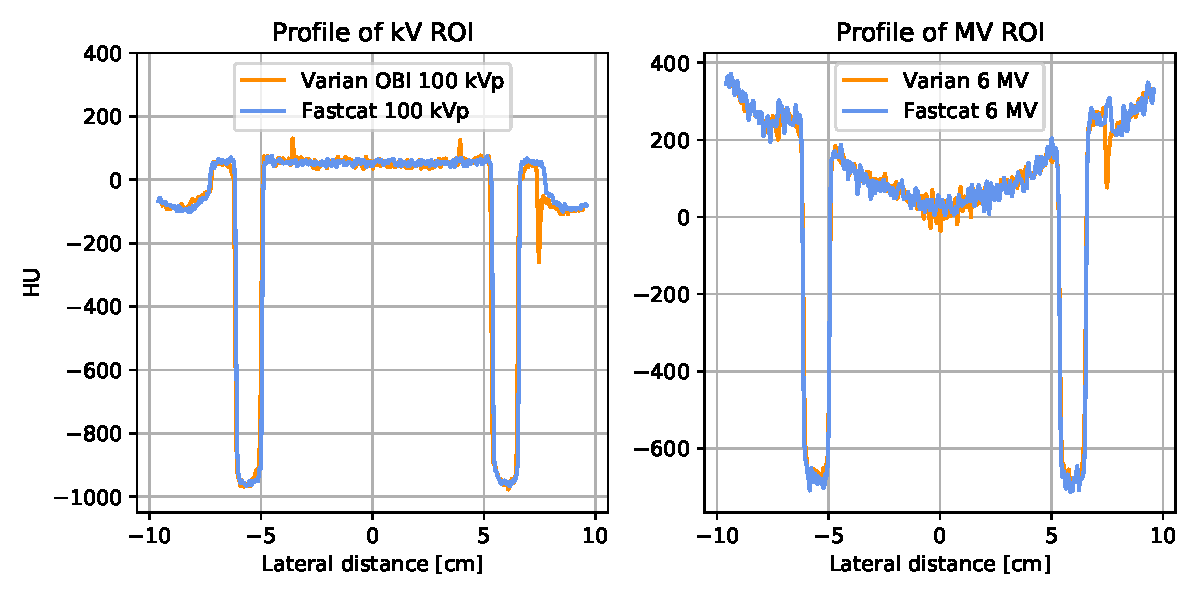
\includegraphics[width=0.75\textwidth, clip]{figures/one_profile.pdf}
  \caption{
  Profiles over the ROI marked in red in Figure \ref{images}. The two peaks at -4/4 cm and the valley at 7 cm correspond to wire ramps and alignment markers in the experimental phantom, respectively. These features were not included in the Fastcat simulations.
  \label{profile} 
    }  %note label inside caption
    \end{center}
\end{figure}

Different features can be seen in the averaged CT images in Figure \ref{images}. The 100 kVp image shows a radial uniformity thanks to the presence of the bowtie filter. However, the image is not completely uniform. The bowtie filter ends just inside the lower density outer layer of the Catphan. This causes non-uniformity in the phantom in this lower density region. A difference between the experimental and Fastcat kV images is a large crescent artifact denoted by a white arrow in Figure \ref{images}. The effect of this artifact can also be seen at the edges of the kV profile in Figure \ref{profile}. In the Varian documentation such artifacts are said to be related to mechanical misalignment between the detector, x-ray tube and bowtie filter. Since Fastcat does not account for this sort of artifact it is not present in the Fastcat image. A dark circle artifact is also present at the center of the 100 kV experimental image. Ring artifacts due to pixel non-uniform response were prevalent in this area and this artifact is due to the accumulation of these ring artifacts and has no physical significance.

In the 6 MV image, the flattening filter causes the beam to be harder in the center of the phantom than the periphery. This leads to cupping in the center of the phantom as seen in both images. Some difference is seen between MV profiles in the center of the phantom in Figure \ref{profile}. This difference may be from ring artifacts or due to the estimation of the flattening filter as Gaussian. 

Overall, the contrast is visibly similar in between both sets of images in Figure \ref{images}. The 100 kVp image has high contrast, clearly differentiating all of the inserts while the 6 MV image has low contrast reflecting the lower number of photo-electric interactions at this energy.

\begin{figure}[ht!]
  \begin{center}
  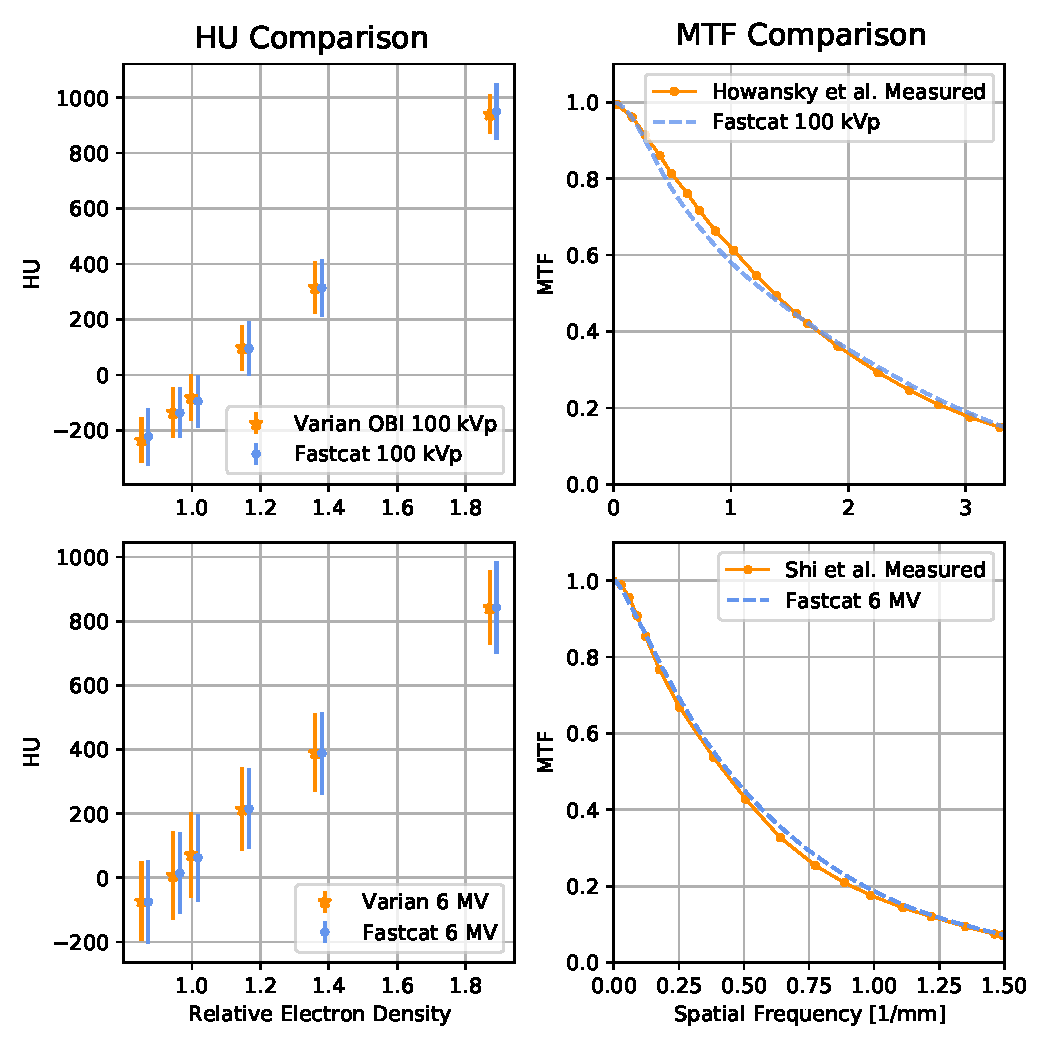
\includegraphics[width=0.75\textwidth, clip]{figures/CNR_MTF.pdf}
  \caption{
  (L) A comparison is demonstrated between the experimental kV and MV CBCTs and the Fastcat simulations in terms of HU values in an experimental and virtual CTP404 module, respectively. (R) Comparison of detector MTFs calculated by Fastcat and based on experimental data presented by Howansky \textit{et al.} \cite{} and Shi \textit{et al.} \cite{Shi2018APerformance} for the kV and MV detector, respectively. The Fastcat 6 MV MTF curve shown is similar to work from Figure 3. in O’Connell and Bazalova-Carter \cite{OConnell2021FastCAT:Simulation} with a slightly larger pixel size of 0.392 mm rather than 0.336 mm.
  \label{HU} 
    }  %note label inside caption
    \end{center}
\end{figure}

\subsubsection{Contrast and MTF}

% Please add the following required packages to your document preamble:
% \usepackage{booktabs}
% Please add the following required packages to your document preamble:
% \usepackage{booktabs}
\begin{table}[]
\caption{kV and MV HU values in CTP404 module, values are in HU while standard deviations are in parentheses.
}
% \vspace{2mm}
\label{table}
\begin{center}
\begin{tabular}{|l|c|c|c|c|c|c|}
\hline
                & PMP        & LDPE       & Polystyrene & Acrylic   & Delrin    & Teflon     \\ \hline
kV Exp.     & -204 (91)  & -102 (102) & -48 (92)    & 135 (91)  & 357 (105) & 995 (87)   \\ \hline
kV Fastcat  & -192 (103) & -104 (91)  & -62 (93)    & 133 (97)  & 356 (102) & 1005 (102) \\ \hline
Abs. Diff.  & 12         & 2          & 14          & 2         & 1         & 10         \\ \hline
MV Exp.     & -70 (124)  & 14 (136)   & 74 (131)    & 219 (129) & 397 (121) & 847 (115)  \\ \hline
MV Fastcat  & -73 (129)  & 17 (126)   & 65 (135)    & 222 (124) & 398 (128) & 850 (144)  \\ \hline
Abs. Diff.  & 3          & 3          & 1           & 3         & 1         & 3          \\ \hline
\end{tabular}
\end{center}
\vspace{10mm}
\end{table}


Looking quantitatively at these images, there is also close agreement. In Figure \ref{HU}, HU values are compared between experimental and Fastcat CBCT images. The HU values in the inserts are shown in Table \ref{table}. HU values for the kV and MV images agreed within 14 and 9 HU values, respectively. The kV HU values were all within the range defined in the Catphan documentation. kV and MV detector MTF was also compared to measurements made by  and Shi \textit{et al.}, respectively. The measurements for the CsI detector were within 4.2\% of measurements by Howansky \textit{et al.} with an average RMSE of 1.7\%. MTF deviated mostly at frequencies between 0.5-1.3 mm$^{-1}$ while agreeing closely at larger spatial frequencies. The MTF measurements for the GOS detector were within 2.5\% of  measurements by Shi \textit{et al.} agreeing well over all spatial frequencies with an average root mean squared error (RMSE) of 0.5\% and a slightly higher MTF at spatial frequencies between 0.5-1.0 mm$^{-1}$.

\subsubsection{CNR and Dose}

CNR was examined in each insert for each of the images seen in Figure \ref{images}. The CNR results are shown in Figure \ref{CNR}. CNR values are summarized in Table \ref{tableCNR}. CNR agreed within 0.4 and 0.2 for the kV and MV images, respectively. CNR as a function of dose was examined as seen in Figure \ref{CNR}. Fastcat CNR values were seen to have average RMSE of 2.6\% and 1.4\% for kV and MV images, respectively. RMSE between experimental and Fastcat CNRs as a function of dose were seen to be 1.19\% and 1.22\%, respectively.

\begin{table}[h!]
\caption{kV and MV CNRs in CTP404 module, standard deviations are in parentheses.
}
% \vspace{2mm}
\label{tableCNR}
\begin{center}
\begin{tabular}{|l|l|l|l|l|l|l|}
\hline
           & PMP       & LDPE      & Polystyrene & Acrylic   & Delrin    & Teflon      \\ \hline
kV Exp.    & 6.1 (.55) & 6.7 (.62) & 6.9 (.72)   & 7.9 (.50) & 8.9 (.56) & 12.0 (1.11) \\ \hline
kV Fastcat & 6.5 (.57) & 6.9 (.54) & 7.1 (.74)   & 7.9 (.46) & 9.1 (.64) & 12.0 (.88)  \\ \hline
Abs. Diff. & 0.4       & 0.2       & 0.2         & 0.0       & 0.2       & 0.0         \\ \hline
MV Exp.    & 6.2 (.34) & 6.7 (.35) & 7.0 (.70)   & 7.8 (.56) & 8.7 (.59) & 11.0 (.74)  \\ \hline
MV Fastcat & 6.4 (.60) & 6.9 (.56) & 7.1 (.76)   & 7.8 (.65) & 8.9 (.66) & 10.8 (.55)  \\ \hline
Abs. Diff. & 0.2       & 0.2       & 0.1         & 0.0       & 0.2       & 0.2         \\ \hline
\end{tabular}
\end{center}
\vspace{10mm}
\end{table}

\begin{figure}[ht!]
  \begin{center}
  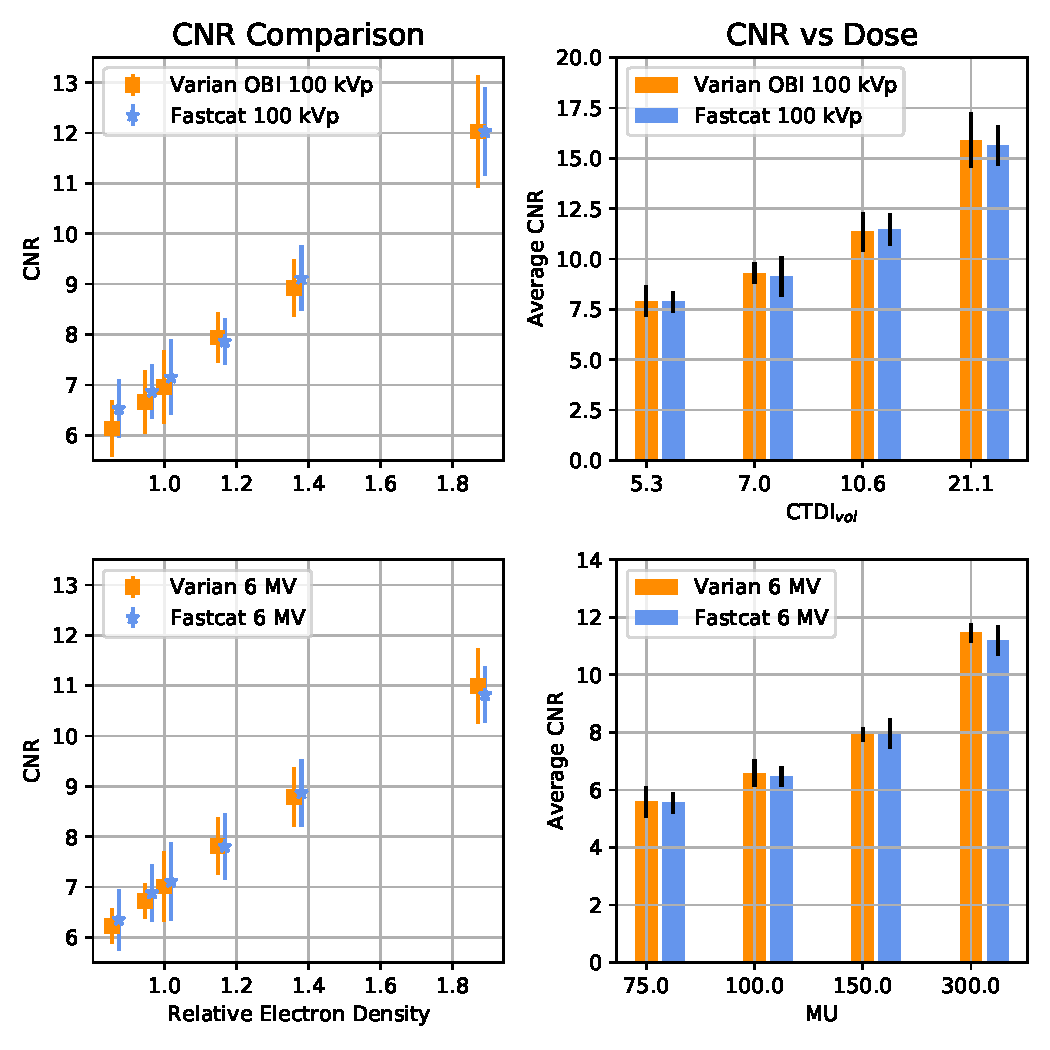
\includegraphics[width=0.75\textwidth, clip]{figures/CNR_dose.pdf}
  \caption{
  (L) A comparison is shown between the Varian Truebeam kV and MV CBCTs and the Fastcat simulated CBCTs in terms of CNR in an experimental and virtual CTP404 module, respectively. (R) CNR is compared between Truebeam CBCTs and Fastcat CBCTs as a function of dose. \label{CNR} 
    }  %note label inside caption
    \end{center}
\end{figure}

\subsubsection{NPS}

NPS was examined in a 100 $\times$ 100 pixel region in the center of each of the images seen in Figure 2. NPS results are shown in Figure \ref{NPS}. NPS agreed within 11 and 14 HU$^2$ mm$^3$ for the kV and MV images respectively. Fastcat and experimental NPS had average RMSEs of 7 and 9 HU$^2$ mm$^3$ with a slightly larger discrepancy at higher spatial frequencies between 0.6 to 1 mm$^{-1}$.

\begin{figure}[ht!]
  \begin{center}
  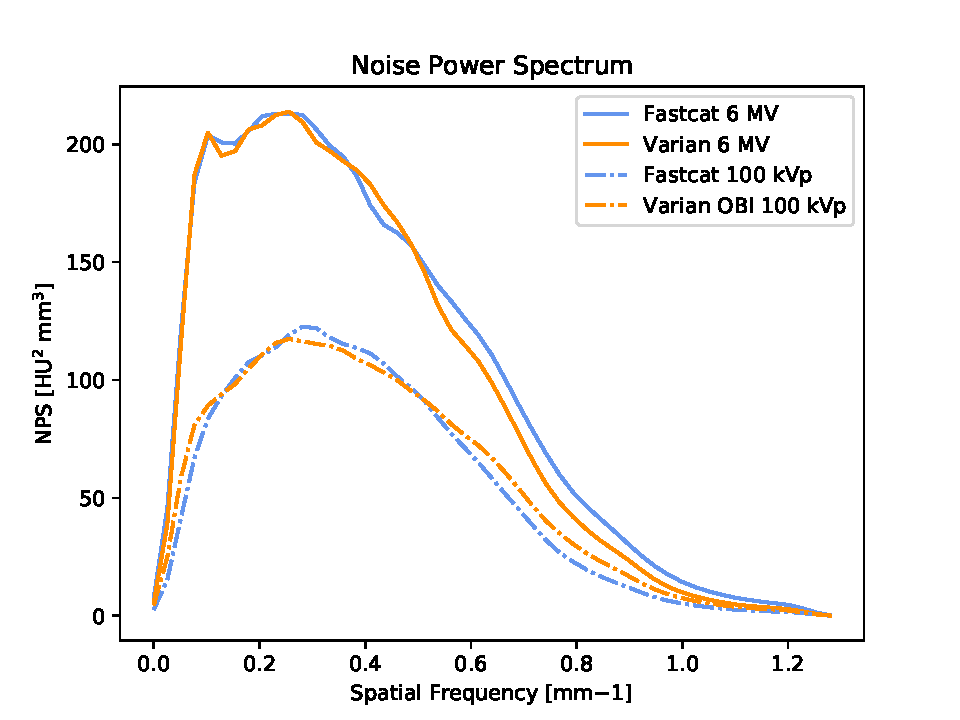
\includegraphics[width=0.75\textwidth, clip]{figures/NPS.pdf}
  \caption{
  NPS in the center of the Catphan 404 module. Calculated from 50 separate 64 $\times$ 64 pixel ROIs in a 100 $\times$ 100 pixel area in the center of the phantom and averaged. \label{NPS}}
    \end{center}
\end{figure}

\subsubsection{Dose and Speed}

Dose was compared between MC simulations and Fastcat using 2 $\times$ 10$^8$ initial photons. Dose was calculated for both the kV and the MV CBCT simulated acquisitions. The mean dose to the entire Catphan for a single projection with the kV beam were 0.416 and 0.426 $\mu$Gy for the MC and Fastcat calculation, respectively. The mean doses to the Catphan for the MV beam were 7.31 and 7.19 $\mu$Gy for the MC and Fastcat calculation, respectively. Thus, there were differences of 2.4\% and 1.6\% between Fastcat and MC dose calculations for kV and MV, respectively. By matching Fastcat and experimental CNRs, the number of Fastcat photons per projection was found to be 9.59 $\times$ 10$^{10}$ and 1.42 $\times$ 10$^{11}$ for the kV and MV images. As a result, the Fastcat mean phantom doses for 887 and 493 projections were 17.52 mGy and 2.566 Gy for the kV and MV simulations, respectively. These values were  consistent with the CTDI of 21.2 mGy and 300 MU reported by the linac for the kV and MV simulations, respectively.


Simulation times were recorded for four Fastcat simulations to estimate the relationship between computation time and the number of projections. Results are shown in Figure \ref{speed}. Computation time scaled linearly with the number of projections for the MV and kV Fastcat simulations with both linear fits having R$^2$ values above 0.999. kV simulations are faster, scaling at 0.37 s/projection while MV simulations scaled at 0.55 s/projection. kV simulations are seen to be more computationally efficient since only ten discrete energies are simulated between 10 and 100 keV while the MV simulation used 18 energies between 10 keV and 6 MeV. All simulated phantoms contained 12 different materials.

The phantom in this study was low resolution in the \textit{z} axis to reduce simulation times. An increase in simulation time can be expected for higher resolution phantoms. For example, using the same parameters as the 6 MV beam in Figure 6 which took 74 seconds to simulate 493 projections, using an isotropic phantom with a voxel size of 0.195 mm takes 108 seconds.

\begin{figure}[h!]
  \begin{center}
 
  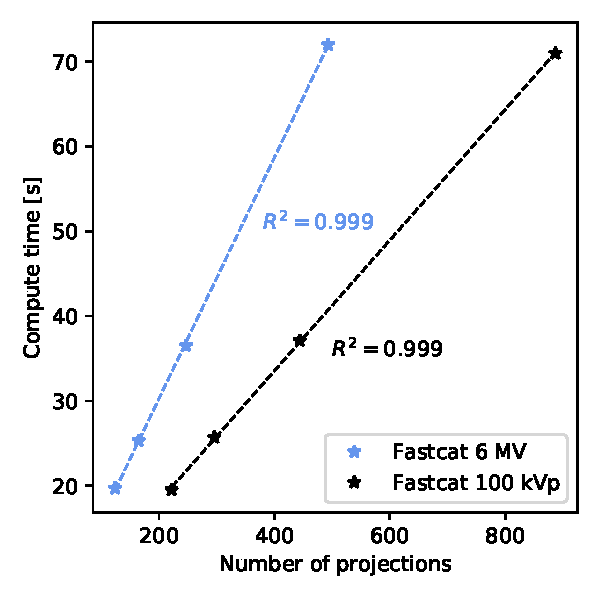
\includegraphics[width=0.5\textwidth, clip]{figures/speed.pdf}
  \caption{A time comparison as a function of the number of projections in a Fastcat CBCT simulation. 
 \label{speed} 
    }  %note label inside caption
    \end{center}
\end{figure}

\subsection{Discussion}

% While the end goal of this platform is to achieve agreement of Fastcat and experimental CBCTs data, this work focuses on agreement between Fastcat simulations and MC simulations as an initial validation.
% Overall, there was a close agreement between Fastcat and MC-generated MV CBCT images and the next step will consist of experimental validation.
\subsubsection{Simulation Validation}
One validated Fastcat result is the MTF of the GOS and CWO detectors, which had a mean error of 1.2\% and 3.5\% of detector measurements performed by Shi \textit{et al.} and Star-lack \textit{et al.} respectively. This comparison lends some validity to the Fastcat simulation method. However, the full MC imaging simulations contains assumptions which may need to be modified to return result consistent with experimental data. These assumptions, such as a spatially uniform cone beams and not generating scatter in the primary and secondary collimators, will perhaps degrade the agreement between Fastcat results and experimental measurements. Further work will assess this fidelity and might lead to adjustments in Fastcat so as to attain the highest possible agreement with experimental data.

Fastcat's agreement with MC image quality metrics is a validation of two assumptions underlying Fastcat: 1) Simulating a phantom at 18 discrete energies, and combining with the weighting described, is sufficient to recreate MC image quality metrics accurately. 2) Scatter does not need to be angularly dependent in a Catphan simulation to generate agreement with the MC image metrics discussed.

Further, scatter generated from a uniform water phantom was an estimate of the scatter generated in a phantom of the same size containing contrast inserts. The nearly identical Fastcat and Topas intensity profiles shown in Figure \ref{one_slice_comparison} explicitly validate this assumption. The difference between Fastcat and Topas for the 6 MV aluminum, 6 MV tungsten, and 120 kVp beams, with respective RMSEs of 0.4, 0.2, and 0.5\%, indicated that a generalized scatter is sufficient to produce intensity profiles within 0.5\% of MC values. Due to the close agreement resulting from the uniform phantom we speculate that a similar agreement would be found for the similar sized XCAT head phantom and further research will investigate this agreement. We should note that for body-sized phantoms, a new scatter model would have to be built.

\subsection{Experimental Validation}

We present and perform a two energy validation of Fastcat, a free open-source CBCT simulator against CBCTs acquired on a Varian Truebeam linac. This simulator performed simulations of high-resolution voxel based phantoms on a desktop computer with 16 GB of memory and an Nvidia RTX 2070 GPU. Simulation times were on the order of a minute to simulate the images used in the validation. Simulated CBCT images demonstrate unprecedented accuracy for their speed, enabling novel application of CBCT simulation in research and clinical workflows. A comparison of Fastcat to four other simulation tools is discussed. DukeSim, CatSim, VOXSI, and gDDR were selected for comparison since they accept voxelized phantoms, use analytical methods to reduce simulation times, and were validated with experimental data.

Compared to the validation of other CT and CBCT simulators, the experimental validation of Fastcat is exceptional in its comprehensiveness and accuracy. The two energy validation presented, using very different imaging systems mitigates possible overfitting resulting from a validation on a single scanner as was conducted for DukeSim, CatSim, and gDRR. VOXSI provides an experimental validation at three tube potentials, however, it uses the same source and detector in each simulation. This might lead to uncertainty in extrapolating the simulator to different detectors and sources, as simulation parameters may be unintentionally specific to the one setup.

Fastcat was experimentally validated with the ubiquitous Catphan 504 phantom and standard imaging metrics such as HU values and CNR. Of the simulation tools discussed, only VOXSI is experimentally validated using a common phantom while other tools were validated using only a single material. VOXSI simulations were within 42 HU of a Gammex RMI 467 tissue characterization phantom (Gammex, Middleton, WI), while Fastcat which was within 14 HU of a comparable Catphan CTP404 module. DukeSim displayed simulated CT images of a Mercury phantom \cite{Wilson2013ASystems}, however neither contrast nor CNR comparisons were shown. This Fastcat validation presents CNR agreement to experimental data with an average RMSE of 2.6\% and 1.4\% in the CTP404 module inserts for kV and MV images, respectively.

Unique among the simulation tools discussed, Fastcat demonstrates agreement with detector MTF. Values were within 4.2\% and 2.5\% of measurements for CsI and GOS detectors, respectively. CatSim and DukeSim use a simple estimation of detector spatial resolution based on neighbouring crosstalk. In reality, scintillating detectors have crosstalk that extends further than their nearest neighbors. Fastcat accounts for this based on the fastEPID framework \cite{Shi2019ADetectors.} which found an 81 $\times$ 81 pixel OSF was necessary to simulate an accurate detector response. VOXSI and gDRR do not include simunelations of the spatial resolution.

Computational efficiency was paramount in Fastcat’s methodology. As such, Fastcat’s computational efficiency compares favorably to other CT and CBCT simulation tools. Direct comparisons currently remain unfeasible as simulation times depend on phantom resolution, processors, noise, and the number of projections, variables which are not always presented in the literature. Nevertheless, qualitative comparisons can be made by examining reported simulation times: Fastcat is estimated to have faster simulation speeds than gDDR, 1 projections of a gDRR high resolution anthropomorphic head phantom with isotropic 512 $\times$ 512 $\times$ 100 voxels with 0.976 mm$^2$ transverse dimensions and 2.5 mm slice thickness took 95.3 s on an Nvidia GTX 590 GPU. Analogously, Fastcat took 28 seconds to simulate 360 views of a similar resolution Catphan 504 phantom with a more powerful Nvidia RTX 2070 GPU. VOXSI is also less computationally efficient than Fastcat, taking 45 seconds to simulate a CT with 512 $\times$ 512 $\times$ 1 voxels, 1024 detectors, and 780 projections, on two Intel Xeon 2.67 GHz processors. Simulations in DukeSim invoke a GPU MC tool to calculate scatter, the scatter calculation speed and total calculation speed thus depend on the desired noise. A sample DukeSim CT simulation with a phantom of 1900 $\times$ 1900 $\times$ 1000 with isotropic voxels of 0.25 mm, 6912 projection images, and 47104 detectors, and 10$^8$ MC photons per projection took about 10 minutes on 4 Nvidia Titan Xp GPUs. In this case the simulation of such a large phantom and the added aspect of the MC noise is considered too different from Fastcat to compare computational efficiencies.


% \begin{figure}[hb!]
%   \begin{center}
%   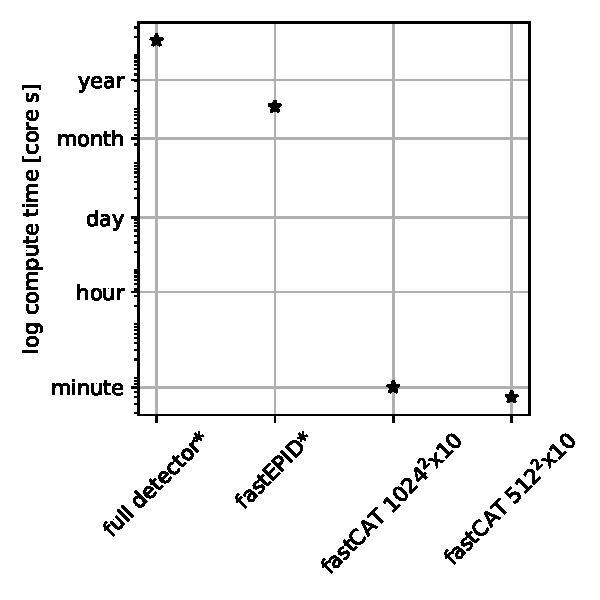
\includegraphics[width=0.5\textwidth]{figures/times.pdf}
%   \caption{
%   {A comparison of the compute time between the different methods discussed.
%   \label{one_slice} 
%     }  %note label inside caption
%     \end{center}
% \end{figure}

% This profile assumes that the coherent scattering does not deviate significantly from its original path. Although this assumption may not hold for lower energy photons it was not seen to significantly impact the results.

\subsubsection{Limitations}

% For example, Fastcat uses a 16 energy approach to quantifying the detector response and scatter kernel. These energies range from 30 keV to 6 MeV which is a good range for most MV and kV imaging applications. One notable exception would be mammography which often focuses on energies below 30 keV. The energy range could be modified to include these applications, however with the geometry of the simulation and the detectors discussed it was seen that photons below 30 keV rarely were detected ($>$0.001\% of fluence). 

% Likewise, 

Fastcat suffers from some rigidity in terms of certain parameters. The detector pixel pitch is not a parameter that can be easily modified from the available built-in detectors as this requires rebinning of MC phasespace files in the case of the GOS detector. These files are too large (up to 2.5 GB in size) to include in the software. For a detector like the CWO, modifying the pixel pitch is even more complicated as the detector septa must be moved and the simulation rerun. The implemented scatter kernels further restricts the use of Fastcat, as scatter is made for the simulation of a 16-cm diameter water phantom and the agreement between Fastcat and MC simulation will degrade for phantoms that are significantly larger or smaller.

Additionally, in the time comparisons, Fastcat would suffer from memory constraints in completing simulations with high resolution reconstructions, while memory would not be a factor in MC simulations. For example, a simulation of the XCAT head phantom with a phantom size of 1024$\times$1024$\times$10 voxels, 360 projections, and a detector size of 124$\times$512 pixels uses 2.6 GB of RAM. Extending this to a full detector of 1024$\times$1024 pixels and a larger phantom one could easily exceed the RAM capacity of most personal computers. This is due to Fastcat memory requirement scaling linearly with the number of detector pixels. Further work will aim to resolve this rigidity. 

We would also like to mention that in the time comparison Fastcat is being compared to a Topas MC simulation without the use of VRTs. Topas was used due to its ability to simulate optical photons. However, Topas as it is a wrapper of Geant4 is seen to be slower than other codes such as EGSnrc in some instances. Sometimes the difference can be by an order of magnitude for common MC simulations \cite{Archambault2015ComparisonBeams}. Likewise, VRTs such as cross section enhancement, interaction forcing, or importance sampling could be used to increase the efficiency of the MC calculation. Thus, it is possible that another MC simulation method could reduce simulation times by about two orders of magnitude as compared to the MC simulations shown in this work.

Likewise, Fastcat is dependent on the TIGRE python package which in turn has a CUDA dependency. This is a limitation of the simulation tool, as many users may not have a CUDA installation, a CUDA capable GPU, or have a GPU at all. Therefore, further work will aim to make a CPU version of Fastcat to increase accessibility.



% \begin{figure}[hb!]
%   \begin{center}
%   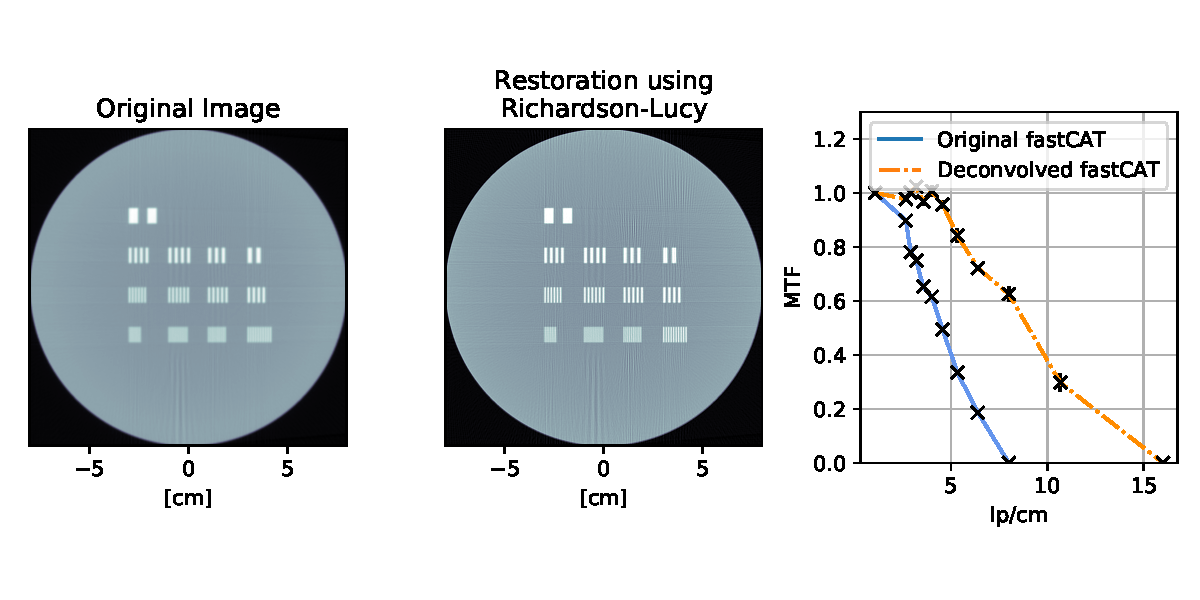
\includegraphics[width=0.5\textwidth]{figures/deconvolution_MTF.pdf}
%   \caption{
%   {Improvement in the overall MTF from the deconvolution process
%   \label{one_slice} 
%     }  %note label inside caption
%     \end{center}
% \end{figure}

% \subsubsection{Future applications}

% Three applications of Fastcat are speculated by the authors: 1) development of new CBCT imaging techniques (the primary goal of this platform), 2) deconvolution of CT images using an approximation of the PSF, and 3) dataset generation for machine learning (ML) deployment. First, Fastcat can be used to quickly asses the effect of various combinations of beam energies and detector types on CBCT image quality. Fastcat greatly decreases the time it takes to simulate these combinations as it can be done in minutes while giving comparable results to MC in terms of image spatial resolution, contrast and CNR. This allows for a greater flexibility in exploring the parameter space for CBCT imaging equipment and protocols. 
% Second, Fastcat generates a PSF for a given beam and detector with an arbitrary focal spot size. If agreement can be achieved between the image MTF of Fastcat and a system experimental data by modification of the focal spot size, one could use the Fastcat PSF to estimate the system PSF. The knowledge of PSF allows one to perform a deconvolution of the image to improve the spatial resolution of CBCT images. In a test case using Richardson-Lucy deconvolution \cite{Richardson1972Bayesian-BasedRestoration,Lucy1974AnDistributions} on a Fastcat MTF phantom (Figure \ref{deconvolution}), CBCT image MTF increased by a factor of two using deconvolution of the projection images. 

% \begin{figure}[h!]
%   \begin{center}
%   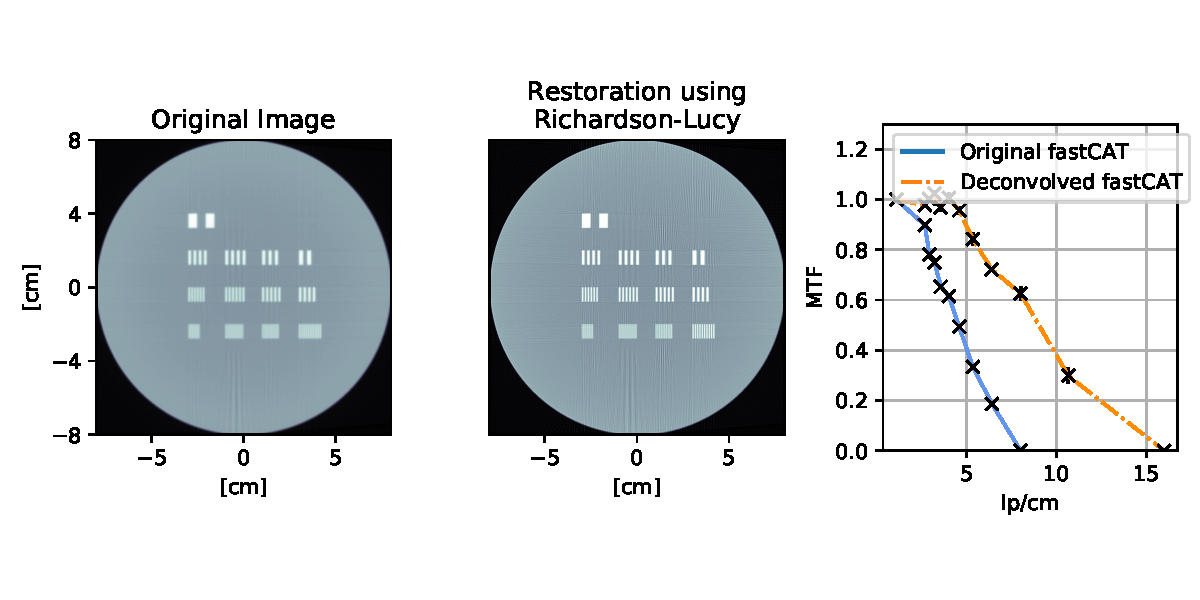
\includegraphics[width=\textwidth,trim={0 0.3cm 0 0},clip]{figures/deconvolution.pdf}
%   \caption{
%   The MTF phantom (L) reconstructed conventionally and (Center) using the Richardson-Lucy deconvolution and the PSF calculated by Fastcat. (R) MTF comparison for the two images. The crosses mark the spatial frequencies in the phantom.
%   \label{deconvolution} 
%     }  %note label inside caption
%     \end{center}
% \end{figure}


% Third, Fastcat could be imagined as a tool to link simulation space to real clinical imaging. This could be done by maintaining a Fastcat model of a clinical imaging setup through adjusting user parameters available in Fastcat to agree with monthly quality assurance (QA) images of a Catphan phantom. A clinic could then use Fastcat to generate arbitrary ML training data personalized to a given machine in terms of contrast and MTF. This overcomes some obstacles that arise in terms of ML algorithms which have to be trained on general datasets and can not necessarily respond to changes in medical imaging equipment output over time. This allows for a more personalized approach between dataset generation that links to clinical QA. The Fastcat simulation method could provide superior performance of ML algorithms and remove risks that ML output would be invalid due to changing machine performance. Automated segmentation of bone CBCT for patient positioning could be suitable for Fastcat, where algorithms could be retrained on adjusted data if drift in QA MTF or contrast indicated a change in image quality.

% Additionally, Figure \ref{XCATs} demonstrates the use of Fastcat with an anthropomorphic phantom to simulating more clinically relevant imaging situations. The use of an anthropomorphic phantom with Fastcat allows users to conduct virtual clinical trials\cite{Abadi2020VirtualCOVID-19}. In a virtual clinical trial, different imaging methods could be compared to ascertain the most successful imaging method for a given clinical situation. This could be used, for example, to asses different CBCT acquisition settings for use in radiotherapy treatment planning.



% \subsection{Conclusion}

% We presented Fastcat: a fast simulation tool for kilovoltage and megavoltage CBCT image generation. Fastcat shows good agreement with measurements with respect to MV beam spatial resolution for a GOS and a CWO detector. The simulation tool was also validated with respect to Monte Carlo simulations using contrast modules of a Catphan 515 phantom. A maximum difference of 16 HU between Fastcat and Monte Carlo simulations was observed for the brain, deflated lung, compact and cortical bone, and adipose tissues inserts. The complete Fastcat CBCT dataset generation for a 512$\times$512$\times$10 and a 1024$\times$1024$\times$10 reconstruction size took 40 and 61 seconds, respectively. This is approximately five orders of magnitude faster than the corresponding Monte Carlo simulations.

